\section{Why GPUs?}


\subsection{Moore’s Law}


\par
Throughout history, computational requirements have primarily revolved around the CPU, a sophisticated component that orchestrates operations across various computing platforms, spanning from desktop computers to laptops and smartphones. The evolution of the modern CPU has been a complex journey, heavily influenced by the rigorous demands set forth by the scientific and HPC domains. Transistors, serving as the foundational units of the CPU, delineate the performance of computers, mobile devices, and other contemporary electronic circuits.

\begin{figure}[!h]
\centering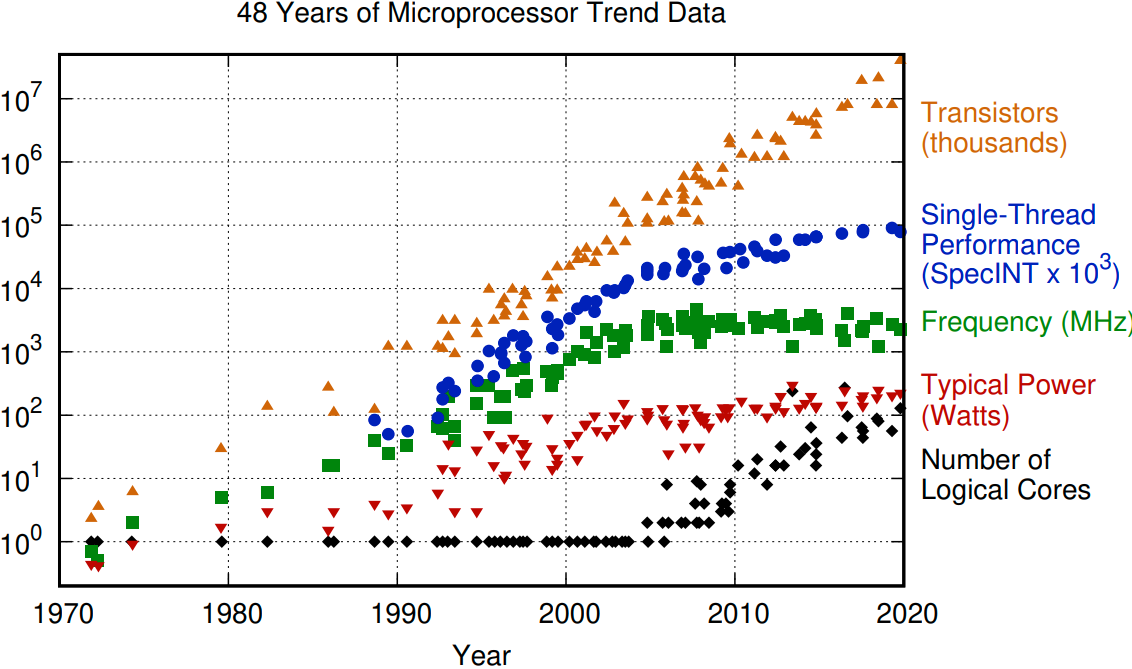
\includegraphics[width=0.8\textwidth]{fig_logo_history/microprocessor_trend.png}
\caption{The Moore’s Law timeline, including Moore's bend with transistors/CPU inflected with multi-core CPUs. Before 2000, the increase in the single core clock frequency was the major source of the increase in the performance. Mid 2000 mark a transition towards multi-core processors. Original data up to the year 2010 collected and plotted by M. Horowitz, F. Labonte, O. Shacham, K. Olukotun, L. Hammond, and C. Batten. New plot and data collected for 2010-2019 by K. Rupp~\cite{microprocessor-trend-data}.}\label{fig:microprocessor_trend}
\end{figure}


\par

\textbf{Moore's Law} posits that the number of transistors in a dense integrated circuit doubles approximately every two years (Fig.~\ref{fig:microprocessor_trend}). With more transistors packed into a smaller space, higher core frequencies can be achieved. Until the early 2000s, CPU manufacturers such as IBM, Intel, and AMD continuously enhanced CPU performance by ramping up clock speeds—16 MHz, 20 MHz, 66 MHz, 100 MHz, and eventually reaching 200, 333, 466 MHz, and so forth. Initially, it seemed feasible to perpetually increase CPU speeds and deliver greater performance each year. However, by the early 2000s, it became evident that the upward trajectory of CPU speeds couldn't continue indefinitely due to constraints on power consumption. Power consumption scales with frequency cubed, leading to a significant slowdown in the growth of core frequency, thereby limiting improvements in the computational performance of single-core CPUs.

\par

The enhancement of computational performance in processing units has been propelled by two primary strategies over the years: 1) Augmenting the performance of individual processors; and 2) More recently, expanding the number of physical cores. Both approaches foster the advancement of parallel computing within the scientific and HPC communities. Indeed, achieving higher performance in a single node often necessitates a more intricate architecture, which can still be attained through techniques like SIMD (single instruction multiple data), branch prediction, and others.


% -------------------------------------------------------------------- %


\subsection{Parallel computing}


\par
Parallel computing, also known as parallel processing or in tandem with parallel programming, involves breaking down a computational problem into smaller subtasks that can be executed concurrently using multiple processing units (Fig.~\ref{fig:comput_serial_parallel}). This approach is indispensable for large-scale projects requiring both speed and accuracy. Although it presents a complex challenge, parallel computing enables developers, researchers, and users to expedite research and analysis compared to sequential processing, where only one task can be processed at a time.


\begin{figure}[!h]
\centering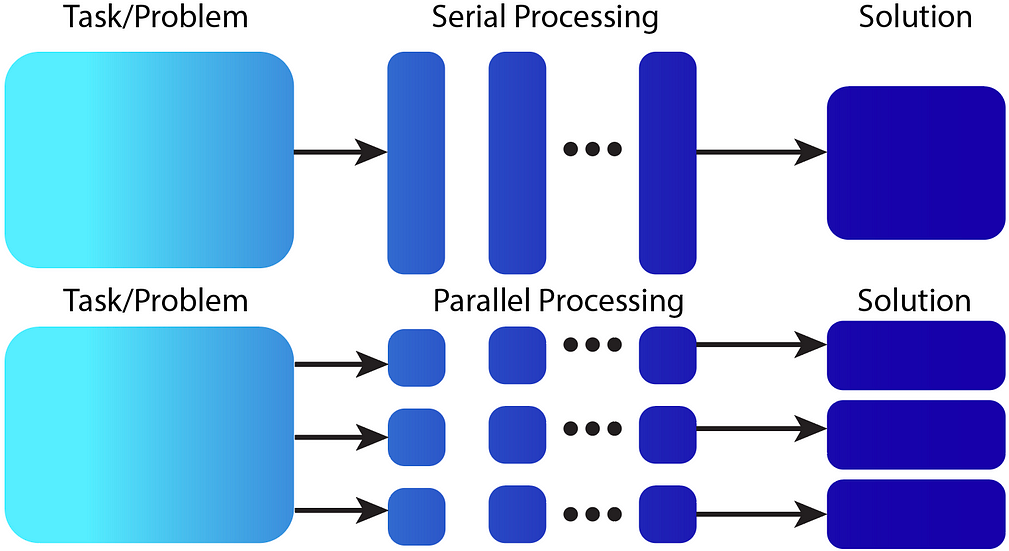
\includegraphics[width=0.8\textwidth]{fig_logo_history/comput_serial_parallel.png}
\caption{Serial processing and parallel computing.}\label{fig:comput_serial_parallel}
\end{figure}


\par

The manner in which a problem is subdivided into smaller subtasks largely hinges on the nature of the problem itself. Broadly speaking, there are two fundamental types of parallelism in applications: \textbf{task parallelism} and \textbf{data parallelism}.
\begin{itemize}
\item Task parallelism emerges when numerous tasks or functions can be executed independently and predominantly in parallel. Task parallelism involves distributing functions across multiple cores.
\item Data parallelism arises when numerous data items can be processed simultaneously. Here, the focus is on distributing the data across multiple cores.
\end{itemize}


\par
More notably, two of the most frequently utilized programming approaches are SIMD and MIMD.
SIMD, or Single Instruction Multiple Data, represents a form of parallel computing closely tied to computer architecture. In a computer with multiple cores, all cores concurrently execute the same instruction stream while operating on different data streams. SIMD is commonly employed for analyzing large datasets based on specified benchmarks. Vector computers are typically classified as SIMD, and most modern computers employ SIMD architecture. One of the primary advantages of SIMD is that programmers can continue to think sequentially while writing code for the CPU, yet achieve parallel speed-up from parallel data operations as the compiler handles the intricacies.
MIMD, or Multiple Instruction Multiple Data, presents another prevalent form of parallel computing and computer architecture, wherein multiple cores operate on multiple data streams, each executing independent instructions. Many MIMD architectures also feature SIMD execution sub-components.

\par

In addition to SIMD and MIMD, computer architecture can also be categorized based on its memory organization, typically into two types: \textbf{multi-node with distributed memory} and \textbf{multiprocessor with shared memory}.
In a multi-node system, large-scale computational engines are constructed from numerous processors interconnected by a network. Each processor possesses its own local memory, and communication between processors occurs by exchanging data stored in their respective local memories over the network. The left figure in Fig.\ref{fig:multinode_vs_multicore} illustrates a typical multi-node system with distributed memory, often referred to as \textbf{clusters}.
Multiprocessor architectures vary in size from dual-processor setups to configurations with dozens or even hundreds of processors. These processors are either directly connected to the same memory (as depicted in the right figure in Fig.\ref{fig:multinode_vs_multicore}), or they share a low-latency link such as PCI-Express or PCIe.
Although shared memory implies a unified address space, it doesn't necessarily mean there is only one physical memory. Such multiprocessors encompass both single-chip systems with multiple cores, known as \textbf{multicore}, and computers comprising multiple chips, each potentially featuring a multicore design.
Multicore architectures have replaced single-core architectures permanently, with the term \textbf{many-core} often used to denote multicore architectures boasting an exceptionally high number of cores, typically numbering in the tens or hundreds.
In recent years, computer architectures have been transitioning from multicore to many-core, with GPUs emerging as a representative hardware for many-core computing.

\begin{figure}[!h]
\centering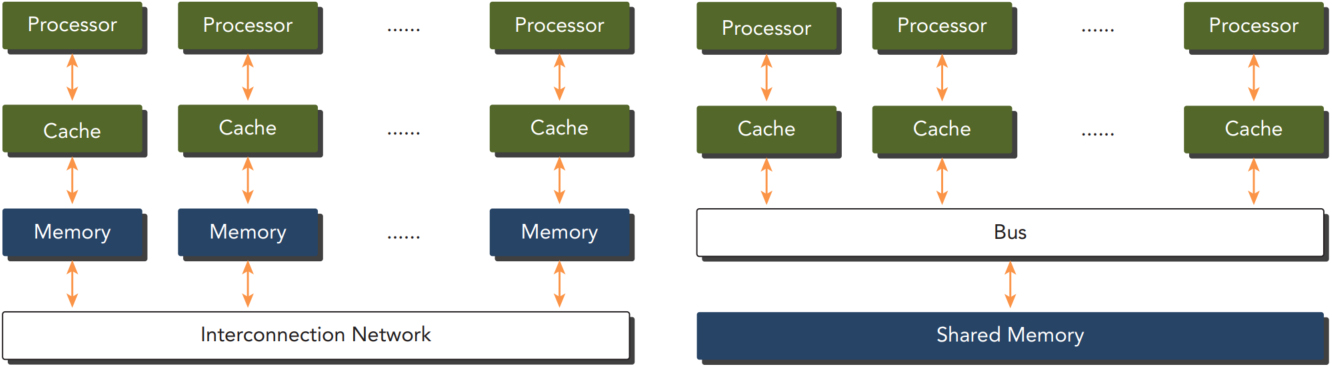
\includegraphics[width=0.9\textwidth]{fig_hardware/multinode_vs_multicore.jpg}
\caption{Two types of computer architectures depending on their memory organization. Left for multi-node with distributed memory and right for multiprocessor with shared memory.}\label{fig:multinode_vs_multicore}
\end{figure}


% -------------------------------------------------------------------- %


\subsection{Graphics processing units}


\par

A GPU, originally conceived as a specialized electronic circuit to expedite computer graphics and image processing tasks, was initially deployed on video cards or embedded within motherboards, mobile phones, personal computers, workstations, and game consoles. However, GPUs have undergone significant evolution in recent years, transforming into potent, general-purpose, fully programmable processors capable of executing both task and data parallel operations. Their many-core architectures make GPUs ideally suited to address massively parallel computing problems~\cite{gpu_wiki}.


% -------------------------------------------------------------------- %


\subsection{Advantages and limitations of CPU and GPU programming}


\par
CPUs have several distinct advantages for modern computing tasks:
\begin{itemize}
    \item Flexibility: a CPU is a general-purpose processor that can handle many tasks, and multitask between multiple activities.
    \item Faster in many contexts: CPUs are faster than GPUs when handling operations like data processing in RAM, I/O operations, and operating system administration.
    \item Precision: CPUs can support mid-range math operations with higher precision than GPUs, which is important for many use cases.
    \item Cache memory: CPUs have a large local cache memory, which lets them handle large sets of linear instructions.
    \item Hardware compatibility: CPUs are compatible with all types of motherboards and system designs, whereas GPUs require specialized hardware support.
\end{itemize}


CPUs have the following disadvantages compared to GPUs:
\begin{itemize}
    \item Parallel processing: CPUs are less adept at tasks that require millions of identical operations because of their limited parallelism.
    \item Slower development: CPUs are a very mature technology that is already reaching the limits of its development, while GPUs have much more potential to improve.
    \item Compatibility: several types of CPUs, including x86 and ARM processors, and software may not be compatible with all types.
\end{itemize}


The unique advantages of GPUs include:
\begin{itemize}
    \item High data throughput: a GPU can perform the same operation on many data points in parallel, so that it can process large data volumes at speeds unmatched by CPUs.
    \item Massive parallelism: a GPU has hundreds or thousands of cores, allowing it to perform massively parallel calculations, such as matrix multiplications.
    \item Suitable for specialized use cases: GPUs can provide massive acceleration for specialized tasks like deep learning, big data analytics, genomic sequencing, and more.
    \item Improved energy efficiency: Compared to CPUs, GPUs can perform more calculations per watt of power consumed, which can result in significant energy savings. This is indeed evident from the Green500 list~\cite{green500}.
    \item Cost-effectiveness: GPUs can be more cost-effective than traditional CPU-based systems for certain workloads.
\end{itemize}


The limitations of GPUs compared to CPUs include:
\begin{itemize}
    \item Difficulty handling complexity: Not all workloads can be efficiently parallelized and accelerated on GPUs. A GPU can struggle with processing tasks that are not well structured. They cannot efficiently process branching logic, sequential operations, or other complex programming patterns. % Certain types of workloads, such as those with irregular data access patterns or high branching behavior, may not see significant performance improvements on GPUs.
    \item Steeper learning curve: Depending on the GPU programming API that you choose, GPU computing could require specialized skills in GPU programming and knowledge of GPU architecture, leading to a steeper learning curve compared to CPU programming. Fortunately, if you study this training material closely you will become productive with GPU programming quickly!
\end{itemize}


\par
GPU computing is not meant to replace CPU computing.
Each approach has advantages for certain kinds of programs.
CPU computing is good for control-intensive tasks, and GPU computing is good for data-parallel computation-intensive tasks.
When CPUs are complemented by GPUs, it makes for a powerful combination.
The CPU is optimized for dynamic workloads marked by short sequences of computational operations and unpredictable control flow; and GPUs aim at the other end of the spectrum: workloads that are dominated by computational tasks with simple control flow. 


\par
If a problem has a small data size, sophisticated control logic, and/or low-level parallelism, the CPU is a good choice because of its ability to handle complex logic and instruction-level parallelism.
If the problem at hand instead processes a huge amount of data and exhibits massive data parallelism, the GPU is the right choice because it has a large number of programmable cores, can support massive multi-threading, and has a larger peak bandwidth compared to the CPU.
The CPU + GPU heterogeneous parallel computing architectures evolved as such a combination ensures that the characteristics of the GPU and CPU complement each other, leading to a full utilization of the computational power of the combined CPU + GPU system.


\par
For the heterogeneous architecture, CPUs and GPUs are discrete processing components connected by the PCI-Express bus (Fig.~\ref{fig:cpu_gpu_architecture}).
The switch from traditional homogeneous CPU systems to current heterogeneous CPU+GPU systems is a milestone in the history of HPC.
\textbf{Homogeneous computing} uses one or more processor of the same architecture to execute an application.
\textbf{Heterogeneous computing} instead uses a suite of processor architectures to execute an application, applying tasks to architectures to which they are well-suited, yielding performance improvement as a result.


\begin{figure}[htbp]
\centering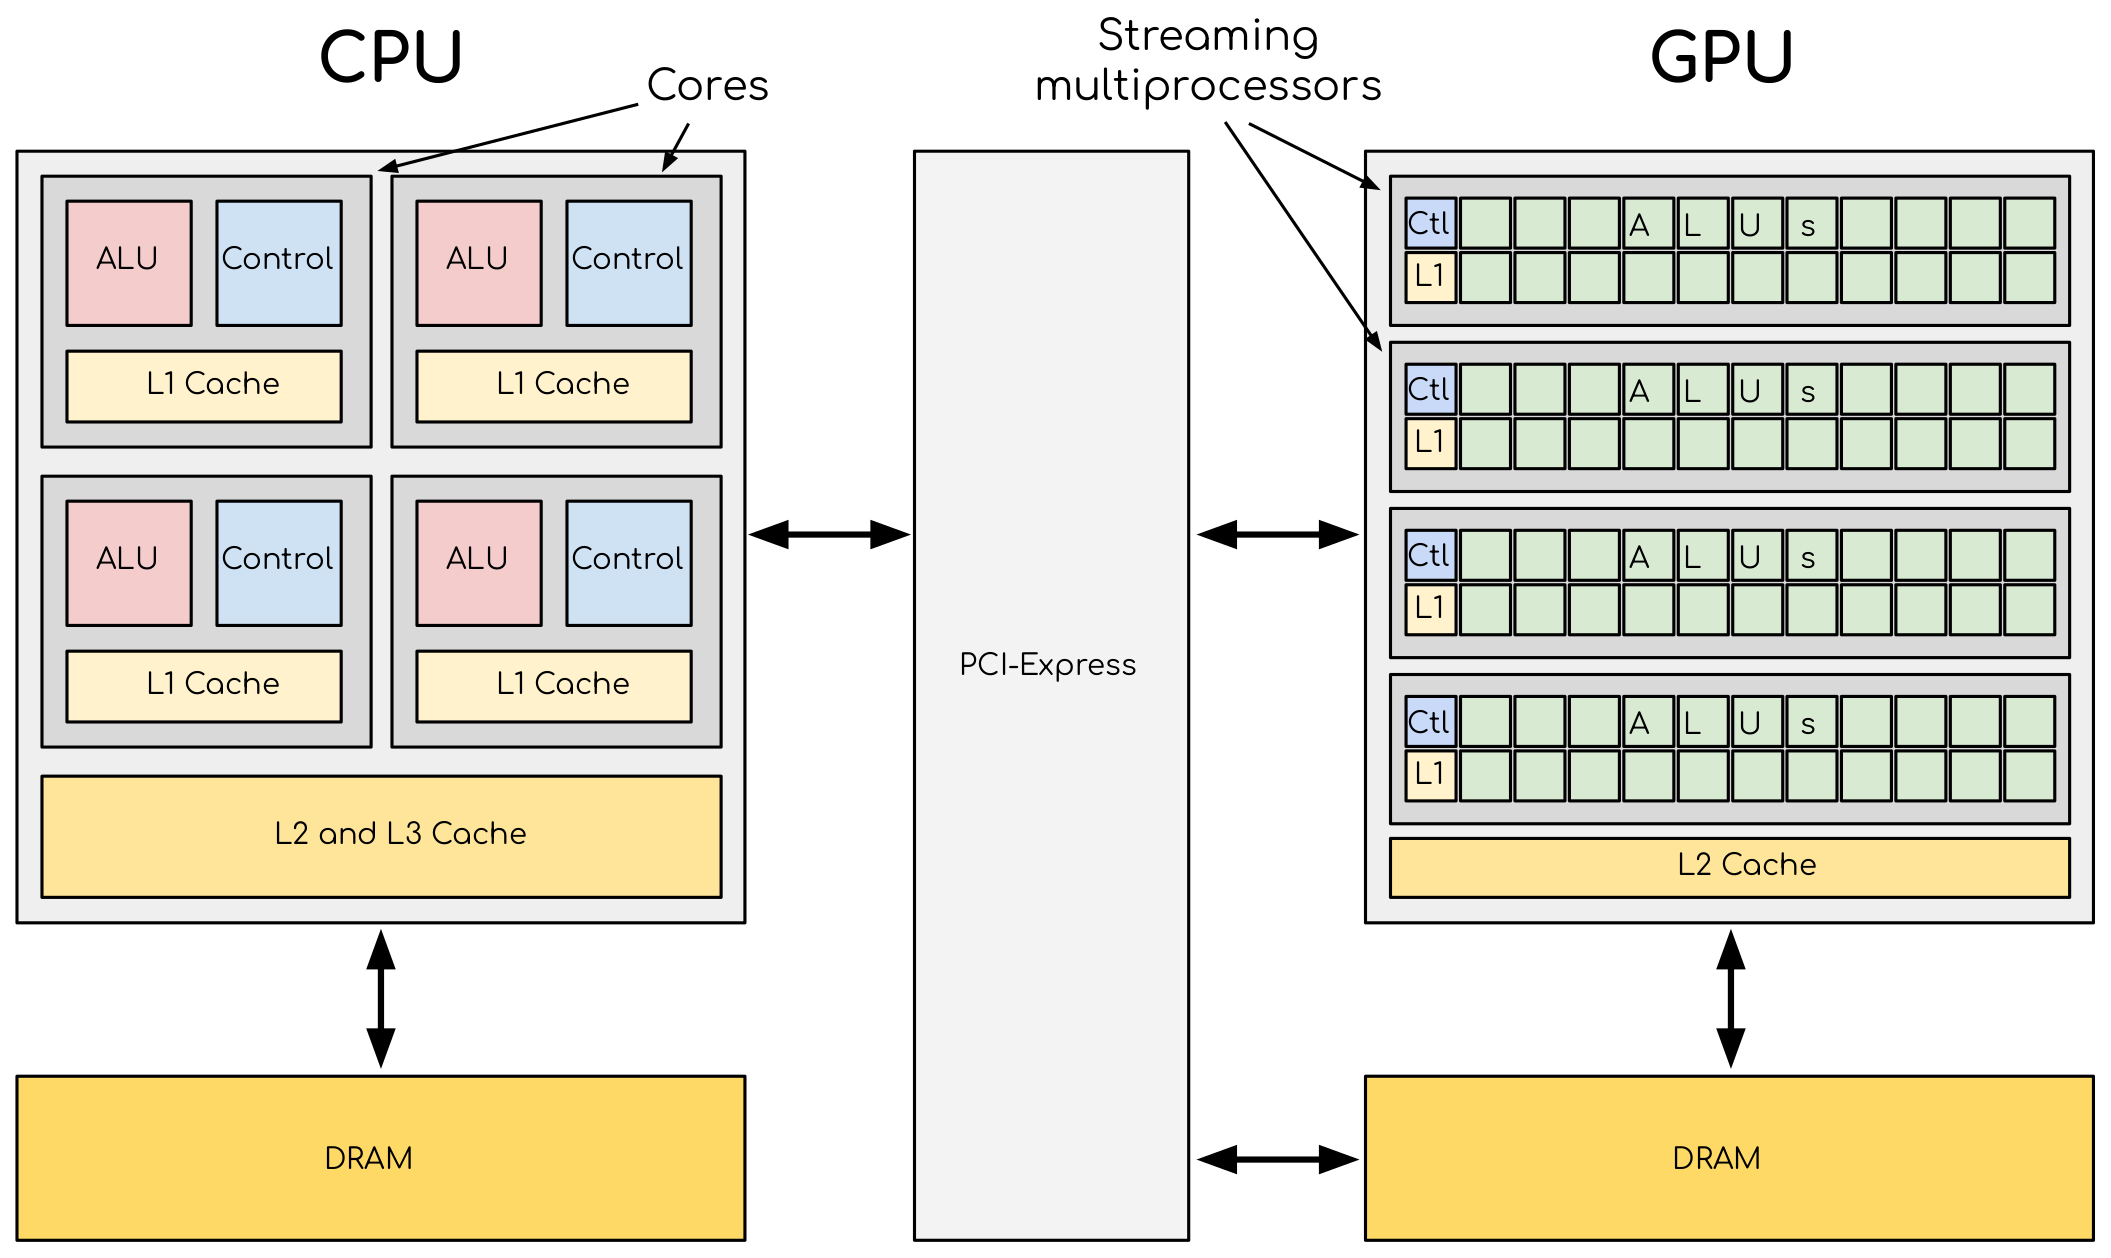
\includegraphics[width=0.8\textwidth]{fig_hardware/cpu_gpu_architecture.png}
\caption{A comparison of CPU and GPU architecture. CPU (left) has complex core structure and pack several cores on a single chip. GPU cores are very simple in comparison, they also share data and control between each other. This allows to pack more cores on a single chip, thus achieving very high compute density.}\label{fig:cpu_gpu_architecture}
\end{figure}


\par
The GPU-enabled heterogeneous computing systems require a heterogeneous programming model that involves both CPU and GPU, where the CPU and its memory are referred to as the~\textbf{host}, and the GPU and its memory as the~\textbf{device}.
Correspondingly, a program running on heterogeneous computing systems consists of two parts, the host code running on CPUs and the device code running on GPUs.
The program executing on a heterogeneous platform is typically initialized by the CPU.
The CPU code is responsible for managing the environment, code, and data for the device before loading compute-intensive tasks on the device.
With computational intensive applications, program sections often exhibit a rich amount of data parallelism. GPUs are used to accelerate the execution of this portion of data parallelism.
Therefore, for optimal performance we need to use both CPU and GPU for computational intensive applications, executing the sequential parts or task parallel parts on the CPU and intensive data parallel parts on the GPU.


\par
To support joint CPU + GPU execution of an application, the three major GPU vendors, NVIDIA, AMD, and Intel, in addition to designing and producing GPUs for HPC, have designed their own computing platforms~\textbf{CUDA} (Compute Unified Device Architecture),~\textbf{ROCm} (Radeon Open Compute), and~\textbf{oneAPI}, respectively.
This way they can offer optimization, differentiation (offering unique features tailored to their devices), vendor lock-in, licensing, and royalty fees, which can result in better performance, profitability, and customer loyalty.
There are also cross-platform APIs (application programming interfaces) such~\textbf{DirectCompute} (only for Windows operating system),~\textbf{OpenCL}, and~\textbf{SYCL}.

% -------------------------------------------------------------------- %


\subsection{The Top500 HPC supercomputers at a glance}


\par
HPC is a set of technologies that enable large-scale, massively parallel computing.
Traditionally, HPC systems were based on CPUs, but modern HPC systems increasingly make use of GPUs.
It is common for HPC servers to combine multiple CPUs and GPUs in one system.


\par
The TOP500 project ranks and details the 500 most powerful non-distributed HPC systems in the world.
This project was launched in 1993 to improve and renew the Mannheim supercomputer statistics, and publishes an updated list of the supercomputers twice a year~\cite{top500_1}.
Fig.~\ref{fig:supercomputer_top5} shows the top-5 HPC systems as of June 2023~\cite{top500_2}, where the columns show:
\begin{itemize}
    \item Cores: Number of processors
    \item Rmax: Maximal LINPACK performance achieved
    \item Rpeak: Theoretical peak performance
    \item Power: Power consumption
\end{itemize}


\begin{figure}[htbp]
\centering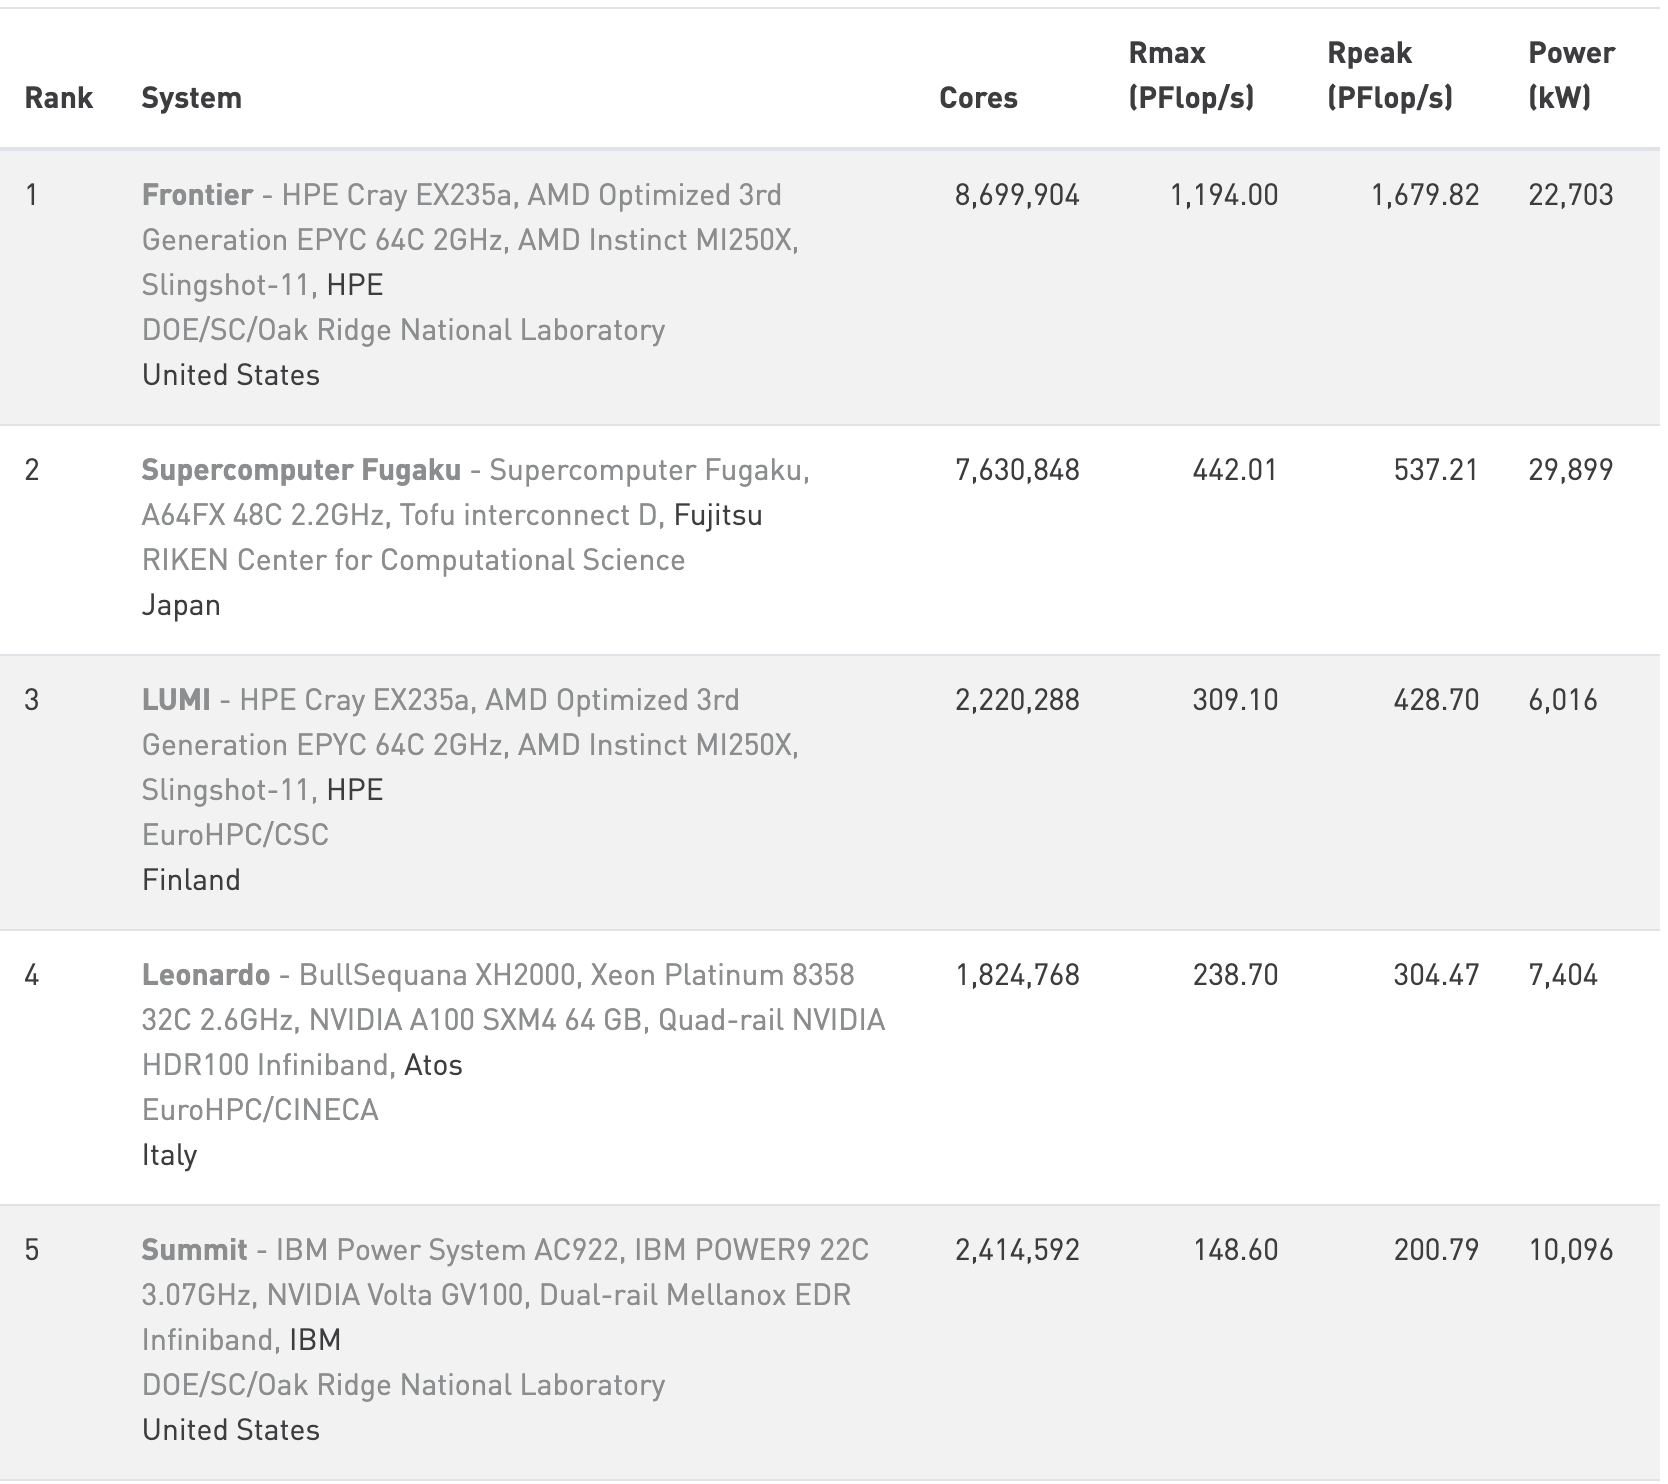
\includegraphics[width=0.8\textwidth]{fig_logo_history/supercomputer_top5.png}
\caption{The top 5 HPC systems on the Top500 list from June, 2023.}\label{fig:supercomputer_top5}
\end{figure}


\par
All systems in the top-5 positions contain GPUs from AMD or NVIDIA, except for the Fugaku system at the RIKEN Center for Computational Science in Kobe, Japan, which instead relies on custom-built Arm A64FX CPUs.
The Frontier system at the Oak Ridge National Laboratory, Tennessee, USA remains the No. 1 system on the TOP500 and is still the only system reported with an HPL performance exceeding one Exaflop/s.
Frontier is based on the latest HPE Cray EX235a architecture and equipped with AMD EPYC 64C 2GHz processors. The system has 8,699,904 total cores, a power efficiency rating of 52.59 gigaflops/watt, and relies on Slingshot-11 interconnect for data transfer.  
The No. 3 and No. 4 HPC systems are the LUMI system at EuroHPC/CSC in Finland and the Leonardo system at EuroHPC/CINECA in Italy, and have HPL scores of 309.1 Pflop/s and 239 Pflop/s, respectively.
The Summit system, also at the Oak Ridge National Laboratory, Tennessee, USA, was launched in 2018 and has a hybrid architecture with each node containing multiple IBM POWER9 CPUs and NVIDIA Volta GPUs all connected together with NVIDIA’s high-speed NVLink.
Each node has over half a terabyte of coherent memory (high bandwidth memory + DDR4) addressable by all CPUs and GPUs plus 800 GB of non-volatile RAM that can be used as a burst buffer or as extended memory.

